% ---
% filename : "telecom_fibre_optique_20260520_004_architecture_ftth.tex"
% id : "telecom_fibre_20260520_004"
% title : "Identification_des_composants_introduction_fibre_optique"
% domain : "TELECOM"
% subdomain : "Fibre_Optique"
% tags : ["TC", "DIT", "suisse", "FTTH", "BEP", "OTO", "limite_propriete"]
% difficulty : 1
% time_solve : 10
% has_octave : false
% author : "om"
% ---
\documentclass[12pt,answers,addpoints]{exam}

% ---------------------------------------------------------
% LANGUE, ENCODAGE, FONTS
% ---------------------------------------------------------
\usepackage[utf8]{inputenc}

% ---------------------------------------------------------
% GÉOMÉTRIE ET MISE EN PAGE
% ---------------------------------------------------------
\usepackage[left=1.7cm,right=1.5cm,top=2cm,bottom=1cm]{geometry}
\usepackage{microtype}
\usepackage{float}
\usepackage{needspace}

% ---------------------------------------------------------
% MATHÉMATIQUES
% ---------------------------------------------------------
\usepackage{amsmath, amssymb, bm, esvect}

\newcommand{\V}{\overrightarrow}
\def\vect#1{\overrightarrow{\strut#1}}
\providecommand{\Degrees}[0]{\ensuremath{^\circ}}

% ---------------------------------------------------------
% UNITÉS ET GRANDEURS (SIunitx)
% ---------------------------------------------------------
\usepackage{siunitx}
\sisetup{output-decimal-marker={,}}
\DeclareSIUnit \var {var}
\DeclareSIUnit \VA {VA}
\DeclareSIUnit \kVA {kVA}
\DeclareSIUnit[quantity-product={}] \degree{\text{\textdegree}}

% Permet la césure dans les nombres avec unités (évite les Underfull \hbox)
%\AllowBreakAtQQ

% ---------------------------------------------------------
% GRAPHIQUES : TikZ + CircuitikZ (sans tkz-fct qui cause des erreurs spath3)
% ---------------------------------------------------------
\usepackage{tikz}
\usetikzlibrary{
	arrows.meta,
	intersections,
	decorations.pathreplacing,
	%	calligraphy,
	positioning
}

\usepackage[european,straightvoltages,EFvoltages]{circuitikz}
\usepackage{pgfplots}
\pgfplotsset{compat=1.12}

% Symbole étoile-triangle personnalisé
\newcommand{\wye}{%
	\mathbin{\tikz[x=1ex,y=1ex]{%
			\draw[line width=.1ex] (0,0)--(45:1)--++(-45:1) (45:1)--++(0,1);
	}}%
}

% ---------------------------------------------------------
% TABLEAUX
% ---------------------------------------------------------
\usepackage{tabularx}
\usepackage{tabu}

% ---------------------------------------------------------
% HYPERLIENS
% ---------------------------------------------------------
\usepackage[colorlinks=true,
menucolor=red,
breaklinks=true,
urlcolor=blue,
linkcolor=blue]{hyperref}

% ---------------------------------------------------------
% COMMANDES PERSONNELLES
% ---------------------------------------------------------
\newcommand\nomauteur{bdminasmorgul@protonmail.com}
\newcommand\dateTe{28.05.2026}
\newcommand\brancheTe{TC}

% ---------------------------------------------------------
% STYLE DE L'EXERCICE
% ---------------------------------------------------------
\pagestyle{headandfoot}
\firstpageheadrule
\runningheadrule

% En-tête avec largeur fixe pour éviter les dépassements
\firstpageheader{\brancheTe\ (\nomauteur)}{Élève : }{\makebox[3.5cm][r]{\dateTe\ \thepage/\numpages}}
\runningheader{\brancheTe\ (\nomauteur)}{Élève : }{\makebox[3.5cm][r]{\dateTe\ \thepage/\numpages}}

% Pied de page
\newcommand{\totalpointtts}{%
	\begin{tikzpicture}[remember picture, overlay]
		\node[anchor=south west, inner sep=0pt, outer sep=0pt]
		at ([xshift=0.5cm,yshift=0.5cm]current page.south west)
		{\rotatebox{90}{Total des points : \numpoints}};
	\end{tikzpicture}%
}

\firstpagefooter{\hspace*{\fill}\totalpointtts}{}{}
\runningfooter{\hspace*{\fill}\totalpointtts}{}{}

% Réglages exam
\printanswers
\addpoints
\pointsinmargin
\bracketedpoints

% ---------------------------------------------------------
% LISTINGS (code)
% ---------------------------------------------------------
\usepackage{xcolor}
\usepackage{listings}

\lstdefinestyle{octavestyle}{
	language=Matlab,
	basicstyle=\ttfamily\small,
	keywordstyle=\color{blue},
	commentstyle=\color{green!50!black},
	stringstyle=\color{red},
	stepnumber=1,
	frame=single,
	breaklines=true,
	breakatwhitespace=true,
	tabsize=4
}

\usepackage{enumitem}
\setlist[enumerate,1]{label=\alph*), ref=\alph*)}
\newenvironment{explication}{%
	\par\noindent\textbf{Explication. }\itshape
}{\par\normalfont}
\renewcommand\partlabel{\arabic{partno}.}
\begin{document}
	\unframedsolutions
	\pointsinmargin
	\bracketedpoints
	
\section*{Préparation TC PQ CFC IELE,PELE}
\begin{questions}
\question 
En tant que planificateur-électricien à Genève, vous réalisez le dossier d'exécution pour le raccordement fibre optique (FTTH) d'un nouvel immeuble locatif. Le maître d'ouvrage souhaite comprendre l'architecture du réseau interne pour définir les limites de maintenance. En vous basant sur le modèle de référence suisse (modèle OFCOM), vous devez identifier deux éléments cruciaux représentés sur votre schéma de principe~:


\begin{parts}
	\part[3] Nommez l'équipement qui sert de point d'entrée du bâtiment et assure la jonction entre le câble de l'opérateur réseau et le câblage interne.
	\part[3] Nommez la prise de raccordement optique finale installée à l'intérieur de chaque appartement.
	\part[12] Nommer les désignations "floutées".
	\begin{center}
		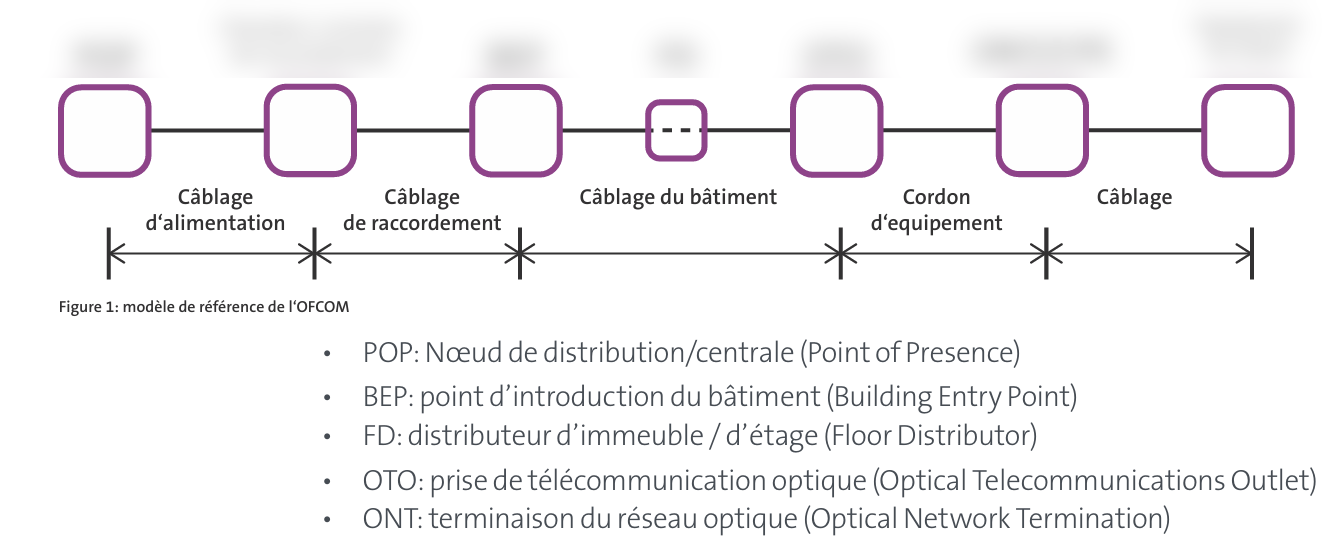
\includegraphics[width=1\linewidth]{OFCOM_MODEL_REF_question.png}
	\end{center}
\end{parts}


\begin{solution}
\textbf{Identification des composants selon le modèle de référence :}
\begin{itemize}
    \item \textbf{a)} : \textbf{BEP} (Building Entry Point). C'est le point d'introduction dans le bâtiment où s'effectue la transition entre le réseau de raccordement extérieur et le câblage inhouse.
    \item \textbf{b)} : \textbf{OTO} (Optical Telecommunications Outlet). Il s'agit de la prise terminale optique installée dans l'appartement, identifiée par un numéro unique (ID OTO) pour le provisionnement des services par le fournisseur.
    \item Modèle de référence de l'OFCOM
    \begin{center}
    	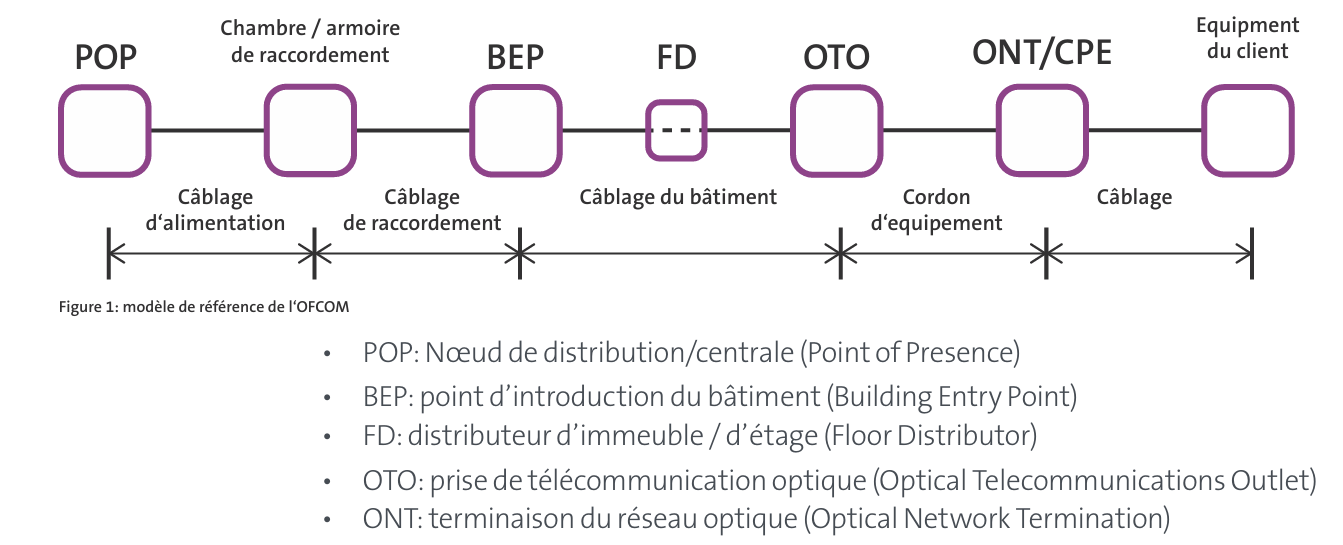
\includegraphics[width=0.8\linewidth]{OFCOM_MODEL_REF_reponse.png}
    \end{center}
\end{itemize}


\end{solution}
\end{questions}
\end{document}